\documentclass{ximera}

\usepackage{algorithm}
\usepackage{algorithmic}
\usepackage{tikz}

\title{Self test}

\begin{document}
\begin{abstract}
A self-evaluation for the University of Leuven's Masters of Artificial
Intelligence program.
\end{abstract}
\maketitle

% using tikz for drawing graphs
\usetikzlibrary{arrows,positioning} 
\usetikzlibrary{arrows,shapes,backgrounds,through,shadows}
\usetikzlibrary{decorations.pathmorphing}
\usetikzlibrary{calc}
\tikzstyle{ugraph}=[line width=1.5pt]
\tikzstyle{cont}=[circle, draw,% a shading that is white at the top...
thick,minimum size=6mm,line width=1pt,>=stealth]  % continuous  node

\subsection*{Mathematics}

% Question 1
\begin{question}
What is the result of $\sum_{i=2}^6 i$?
\begin{solution}
The sum is equal to \answer{20}.
\end{solution}
This sum could be computed via
\[
\sum_{i=2}^6 i = 2 + 3 + 4 + 5 + 6,
\]
or by using the formula
\[
\sum_{i=1}^n i = \frac{n(n+1)}{2}.
\]
\end{question}

% Question 2
\begin{question}
What is  the result of $\prod_{i=2}^{5} i$ ? 
\begin{solution}
The product is equal to \answer{120}.
\end{solution}
$\prod_{i=2}^5 i = 2 \times 3 \times 4 \times 5 = 120$
\end{question}

% Question 3
\begin{question}
What is  the result of  $\prod_{i=1}^5 2^i$  ? 
\begin{solution}
The product is equal to \answer{32768}.
\end{solution}
\begin{align*}
\prod_{i=1}^5 2^i &= 2^1 \times 2^2 \times 2^3 \times 2^4 \times 2^5 \\
&= 2^{1 + 2 + 3 + 4 + 5} \\
&= 2^{15} \\
&= 32768. 
\end{align*}
\end{question}

% Question 5
\begin{question}
What is  the result of  $\log_2 2^k 4^m$  ? 
\begin{solution}
The answer is \answer{$k+2m$}.
\end{solution}
\begin{align*}
\log_2{2^k 4^m} &= \log_2{2^k} + \log_2{4^m} \\
&= k \log_2{2} + m \log_2{4} \\
&= k + 2m.
\end{align*}
\end{question}

\subsection*{Combinatorics}

% Question 6
\begin{question}
In a group of 15 people, everyone shakes hands with everyone else.  How many handshakes are there? 
\begin{solution}
The answer is \answer{105}.
\end{solution}
Every handshake requires two individuals. So the total number of handshakes is equal to the number of ways that we could pick 2 individuals from a group of 15:
\[
\binom{15}{2} = \frac{15!}{(15 - 2)! \cdot 2!} = 105
\]
\end{question}

% Question 7
\begin{question}
A Web search query returns ten answers. How many possible ways are there to rank these ten answers?
\begin{solution}
There are \answer{3628800} ways to rank the answers.
\end{solution}
The possible ways to rank these ten answers are equal to the number of permutations of 10 objects, which is $10! = 3628800$.
\end{question}

% Question 8
\begin{question}
How many subsets are there of $\{1, ... , 100\}$ that do not contain an even number ? 
\begin{solution}
There are \answer{$2^{50}$} subsets.
\end{solution}
Each subset of $\{1 , \ldots , 100\}$ which does not contain an even number is a subset of $\{1, 3, 5, \ldots , 97, 99\}$. So it would suffice to count the number of subsets of $\{1, 3, 5, \ldots , 97, 99\}$. We know that a set containing $n$ elements has $2^n$ subsets (including the empty subset). So the answer is $2^{50}$.
\end{question}

% Question 9
\begin{question}
10 toys are in a box.  A child can choose 3 of them.  How many different choices can it make (disregarding the order in which it chooses the toys)?  
\begin{solution}
There are \answer{120} choices.
\end{solution}
The order is not important, hence the answer is
\[
\binom{10}{3} = \frac{10!}{(10-3)! \cdot 3!} = 120
\]
\end{question}

\subsection*{Probability}

% Question 10
\begin{question}
Box A contains balls with numbers from 1 to 6.  Box B contains balls numbered 1 to 4.   I draw a random ball from A and one from B.  What is the probability the sum of both numbers is 7?
\begin{solution}
The answer is \answer{$\frac{1}{6}$}.
\end{solution}
Let's show each outcome with an ordered pair (in which the first element shows the number of first ball and the second element shows the number of the second ball). All possible outcomes are listed below (The outcomes with a sum of 7 are specified with boldface):
\[
\begin{matrix}
(1,1) & (2,1) & (3,1) & (4,1) & (5,1) & \textbf{(6,1)} \\
(1,2) & (2,2) & (3,2) & (4,2) & \textbf{(5,2)} & (6,2) \\
(1,3) & (2,3) & (3,3) & \textbf{(4,3)} & (5,3) & (6,3) \\
(1,4) & (2,4) & \textbf{(3,4)} & (4,4) & (5,4) & (6,4)
\end{matrix}
\]
\[
Pr (\text{sum = 7}) = \frac{N(\text{sum = 7})}{N(\text{total})} = \frac{4}{24} = \frac{1}{6}
\]
\end{question}

% Question 11
\begin{question}
Box A contains 5 white and 2 black balls.   Box B contains 3 white and 3 black balls.  Someone chose a box randomly (1/2 chance each) and took a random ball from it.  It is black.  What is the probability that the ball was taken from box B?
\begin{solution}
The answer is \answer{$\frac{7}{11}$}.
\end{solution}
Using Bayes rule, we have:
\begin{align*}
Pr (\text{box B} | \text{black}) &= \frac{Pr(\text{black} | \text{box B}) Pr(\text{box B})}{Pr(\text{black} | \text{box B}) Pr(\text{box B}) + Pr(\text{black} | \text{box A}) Pr(\text{box A})} \\
&=\frac{(\frac{3}{6}) \times (\frac{1}{2})}{(\frac{3}{6}) \times (\frac{1}{2}) + (\frac{2}{7}) \times (\frac{1}{2})} = \frac{7}{11}
\end{align*}
\end{question}

% Question 12
\begin{question}
There are two different train connections between cities A and B.  One goes via C, the other via D.  30\% of all trains go via C; among these, 10\% are delayed upon arrival.  70\% go via D; among these, 5\% are delayed.   A train from A arriving in B is delayed.  What is the probability it went via C?
\begin{solution}
The answer is \answer{$\frac{6}{13}$}.
\end{solution}
Using Bayes rule,
\begin{align*}
Pr (\text{via C} | \text{delayed}) &= \frac{Pr(\text{delayed} | \text{via C}) Pr(\text{via C})}{Pr(\text{delayed} | \text{via C}) Pr(\text{via C}) + Pr(\text{delayed} | \text{via D}) Pr(\text{via D})} \\
& = \frac{(0.1)(0.3)}{(0.1)(0.3) + (0.05)(0.7)} = \frac{6}{13}
\end{align*}
\end{question}

% Question 13
\begin{question}
Someone has rolled two dice.  Given that the total is even, what is the probability that it is less than 9?
\begin{solution}
The probability of this event is equal to \answer{$\frac{7}{9}$}.
\end{solution}
Rolling two dice has 36 possible outcomes. Outcomes with a total smaller than 9 are listed below. Among these outcomes, those with an even sum are specified by boldface:
\begin{equation*}
\begin{matrix}
\mathbf{(1,1)} & (1,2) & \mathbf{(1,3)} & (1,4) & \mathbf{(1,5)} & (1,6) \\
(2,1) & \mathbf{(2,2)} & (2,3) & \mathbf{(2,4)} & (2,5) & \mathbf{(2,6)} \\
\mathbf{(3,1)} & (3,2) & \mathbf{(3,3)} & (3,4) & \mathbf{(3,5)} && \\
(4,1) & \mathbf{(4,2)} & (4,3) & \mathbf{(4,4)} &&& \\
\mathbf{(5,1)} & (5,2) & \mathbf{(5,3)} &&&& \\
(6,1) & \mathbf{(6,2)}
\end{matrix}
\end{equation*}
Using Bayes rule,
\begin{equation*}
Pr (\text{less than 9} | \text{even}) = \frac{Pr(\text{less than 9}, \text{even})}{Pr(\text{even})} = \frac{(\frac{14}{36})}{(\frac{18}{36})} = \frac{7}{9}
\end{equation*}
\end{question}

% Question 14 %
\begin{question}
A lottery ticket costs \$5. 
There is no limit to the number of tickets that can be sold, and each sold ticket has a probability of 2\% of winning \$100.
You buy three tickets, what is your expected payout?

\begin{solution}
The answer is \answer{-9}.
\end{solution}

The expected payout of three tickets is equal to the sum of expected payout of each of three tickets. 
\begin{equation*}
E[X_1 + X_2 + X_3] = E[X_1] + E[X_2] + E[X_3] = 3 \times E[X]
\end{equation*}

\begin{equation*}
E[X] = -5 + \left(Pr(X = 100) \times (100) + Pr(X = 0) \times (0)\right) = -5 + 0.02 \times 100 = -3
\end{equation*}
Hence the expected payout of three tickets would be $3 \times -3 = -9$.
\end{question}


\subsection*{Algebra}

% Question 17
\begin{question}
Solve for $x_2$ in the following system of equations:
\begin{eqnarray*}
-2x_1 + 4x_2 & = &-6\\
3x_1  - 9x_2 & = & 12 
\end{eqnarray*}
\vspace*{13pt}
\begin{solution}
The value of $x_1$ is \answer{1} and the value of $x_2$ is \answer{-1}.
\end{solution}
Multiplying the first equation by 3 and the second one by 2, we'll get the following equivalent system:
\begin{alignat*}{2}
 -6  x_1  + 12  x_2 & = -18 \\
 6  x_1  - 18  x_2 & = 24
\end{alignat*}
By summing these two equations we'll get $x_2 = -1$, and by replacing this value for $x_2$ in any of the equations, we'll obtain $x_1 = 1$.
\end{question}

% Question 18
\begin{question}
Multiply the following matrices together:
%\begin{equation}
\[ \left( \begin{array}{cc}
1 & 2 \\
3 & 5 \\
2 & 8
\end{array} \right)
%
\left( \begin{array}{ccc}
2 & 6 & 1 \\
3 & 3 & 3
\end{array} \right)
\]
\begin{solution}
% TODO (Behrouz) add matrix-format solution here
\end{solution}
This is the formula for multiplication of two matrices $A_{m \times n}$ and $B_{n \times p}$:
\[
    (AB)_{ij} = \sum_{k=1}^n A_{ik}B_{kj}. 
\]
Using this formula, we could compute the multiplication of the two given matrices:
\[
\begin{pmatrix}
8 & 12 & 7 \\
21 & 33 & 18 \\
28 & 36 & 26
\end{pmatrix}
\]
\end{question}

\subsection*{Algorithms}

% Question 19
% TODO (Behrouz) Verify if this is the right way of putting multiple-section questions
\begin{question}
Consider the algorithm below.
\begin{algorithm}
\caption{Function(Array $A$)}
\begin{algorithmic}
  \FOR{$i = 1$ to $A$.length}
  \FOR{$j = 1$ to $A$.length--i}
  \IF{$A[i+1] < A[i]$}
  \STATE $temp = A[i]$
  \STATE $A[i] = A[i+1]$
  \STATE $A[i+1] = temp$
  \ENDIF
  \ENDFOR
  \ENDFOR
  \STATE output $A$
\end{algorithmic}
\end{algorithm}

% part 1 of question
If the algorithm is invoked on the array $[ 5~~ 7~~ 3~~ 9]$ what is the output of the algorithm?
\begin{solution}
% TODO (Behrouz) Change this into a row vector with constant #columns
The output is \answer{$ [3 \quad 5 \quad 7 \quad 9] $}.
\end{solution}

% part 2 of question
What does the algorithm do? 
% TODO (Behrouz) Verify if this is a correct implementation of free-response
\begin{free-response}
\end{free-response}
This algorithm sorts the input array using a technique called bubble sort.

% part 3 of question
Given an array with ten elements, how many comparisons (that is, $<$) operations does the following piece of code perform?
\begin{solution}
There are \answer{$45$} comparisons.
\end{solution}  
The number of iterations of the inner loop starts with value 9 and gradually decreases to 1. So the total number of comparisons is $ 9 + 8 + \ldots + 2 + 1 = 45$.

% part 4 of question
Can you generalize your answer such that it gives an upperbound on the number of comparison operations for an array of length $n$?
\begin{solution}
The smallest upper bound (expressed as a function of $n$) is \answer{$n^2$}.
\end{solution}
\begin{hint}
Are you familiar with asymptotic analysis of algorithms (especially the Big-$\Theta$ notation)? 
\end{hint}
For an array of length $n$, the number of iterations of inner loop starts with value $n-1$ and gradually decreases to 1. So the total number of iterations would be $(n-1) + (n-2) + \ldots + 1 = \frac{n(n-1)}{2}$. This indicates that the running time of this algorithm is of $\Theta(n^2)$.
\end{question}

% Question 21
\begin{question}
What is the maximal number of leaves that a sorted binary tree with depth $4$ can possess?
\begin{solution}
The answer is \answer{$16$}.
\end{solution}
The maximal number of nodes at depth-level $d$ of a binary tree is $2^d$. So the answer to this question is $2^4 = 16$. 
\end{question}

% Question 22
\begin{question}
Order the following functions according to their growth-rate (use the theory of big-Oh notation). Put the slower growing functions first.

$ n^7, 8n!, 5 \log_2 n,~ 3n, 2^n, ~ 7.5 n\log_2 n, ~ 6 n^2$ 

% TODO (Behrouz) Present the solution as a row vector 
\begin{solution}
\end{solution}
\begin{equation*}
5 \log_2^n \prec 3n \prec 7.5 n \log_2{n} \prec 6n^2 \prec n^7 \prec 2^n \prec 8n!
\end{equation*}
\end{question}

\subsection*{Boolean Logic}

% Question 23
\begin{question}
Which of the following statements are correct?
\begin{solution}
\begin{multiple-choice}
\choice[correct]{not(A and B) is true whenever A is false or B is false}
\choice[correct]{not (A or B) is true if and only if (not A and not B) is true}
\choice{not (A or B) is true if and only if  (not A or not B) is true}
\choice[correct]{not (A and B) is true whenever A is false}
\end{multiple-choice}
\end{solution}
\end{question}

% Question 24
\begin{question}
Simplify the following boolean expression: \\
(A and B) or (A and B and C) or (A and B and C) or (A and B and C and D) or (A and B and C and D).
\begin{solution}
% TODO (Behrouz) There should be a better way of doing this
The answer is \answer{A and B}. 
\end{solution}
\end{question}

% Question 25
\begin{question}
Is the following boolean expression satisfiable, i.e., is there an assignment to the variables $A$ and $B$ so that the following expression evaluates to true?  \\
\\
A or (not A and B) or (not A and not B and C)\\
\\
If so, state one.
\begin{solution}
% TODO (Behrouz) This way of presenting the answer reveals the answer to the first part. Fix it!
% TODO (Behrouz) This is not a correct specification of solution; as any assignment to B and C would be also valid. Is there a way to specify more than one correct answer?
By assigning value \answer{true} to \emph{A} and \answer{false} to \emph{B} and \answer{false} to \emph{C}, the equation evaluates to true.
\end{solution}
\end{question}

\subsection*{Set theory}

% Question 26
\begin{question}
% TODO (Behrouz) check to see if it is possible to put it as some sort of multiple-choice question
Which of the following statements are always true (AT), which are always false (AF), and which may be true or false depending on the sets (TF) ?
\begin{solution}
$(C \setminus A) \setminus B = C \setminus (A \cup B)$ is \answer {AT}. \ \\
$ C \setminus (A \cup B) = (C \setminus A)  \cap (C \setminus B)$ is \answer {AT}.
\end{solution}
\end{question}

% Question 27
\begin{question}
Let $A$ be the set of all animals, $B$ the set of all birds, and $F$
the set of all flying animals. Which of the following statements are correct?
\begin{solution}
\begin{multiple-choice}
\choice[correct]{$B\cap F$ is the set of all birds that can fly.}
\choice[correct]{$B\setminus F$ is the set of all birds that do not fly.}
\choice{$F\subseteq B$.}
\end{multiple-choice}
\end{solution}
\end{question}

% Question 28
\begin{question}
Simplify $(A \cap B) \cup (A \cap B^C)$ where $B^C$ is the complement of $B$.
\begin{solution}
The answer is \answer{A}. \\
$(A \cap B) \cup (A \cap B^C) = A \cap (B \cup B^C) = A \cap \mathbb{U} = A$
\end{solution}
\end{question}

% Question 29
\begin{question}
A survey of 500 students taking one or more courses in algebra, physics and statistics during one semester revealed
the following number of students in the indicated subjects : 
329 in Algebra, 186 in Physics, 295 in Statistics, 83 taking Algebra and Physics, 217 Algebra and Statistics, and 63 Physics and Statistics.
How many students took all three subjects ? 
\begin{solution}
The answer is \answer{$53$}. 
\end{solution}

Let us denote the set of students taking courses Algebra, Physics, and Statistics by letters $A$, $P$, and $S$, respectively. We have this information about cardinality of these three sets:

\begin{equation*}
	\begin{array}{lll}
	 |A| = 329							& |P| = 186				& |S| = 295 \\
	 |A \cap P| = 83				& |A \cap S| = 217	& |P \cap S| = 63 \\
	 |A \cup P \cup S| = 500	& &
	\end{array}
\end{equation*}

According to the principle of inclusion-exclusion, for three sets A, P and S we have:
\begin{align*}
|A \cup P \cup S| &= |A| + |P| + |S| - |A \cap P| - |A \cap S| - |P \cap S| + |A \cap P \cap S|\\
|A \cap P \cap S| &= 500 - 329 - 186 - 295 + 83 + 217 + 63 = 53
\end{align*}
\end{question}

\subsection*{Calculus}

% Question 30
\begin{question}
If $\frac{df}{dx}$ is the derivative of $f$, what is the value of $\frac{df}{dx}(4)$ assuming that 
$f(x) = 5x^2 +3x$ 

\begin{solution}
$\frac{df}{dx}(4)$ is equal to \answer{$43$}.
\end{solution}

$f(x) = 5x^2 + 3x \Rightarrow f'(x) = 10 x + 3 \Rightarrow f'(4) = 43$
\end{question}

% Question 31
\begin{question}
What is the value of $f(5) $ assuming that $f(x) = \int_1^x 3t ~dt$?
\begin{solution}
The answer is \answer{$36$}.
\end{solution}
$f(5) = \int_1^5 3t dt = \left. \frac{3t^2}{2} \right|_1^5 = \frac{72}{2} = 36$
\end{question}

\subsection*{Linear Algebra}

% Question 33
\begin{question}
True or false?  When the dot product of two vectors is negative, the angle between them is between 90 and 270 degrees.
\begin{solution}
\begin{multiple-choice}
\choice[correct] {true}
\choice {false}
\end{multiple-choice}
\end{solution}
Since the lengths of two vectors are always non-negative, a negative dot product indicates an angle with negative cosine. The range of angles with a negative cosine are those between 90 and 270 degrees.
\end{question}

% Question 34
\begin{question}
Given the vectors $u$ and $v$, give a matrix $M$ that transforms them into $u'$ and $v'$; that is, find $M$ such that $M u=u'$ and $M v=v'$.
% TODO (Behrouz) the vectors in this image should be transposed
% TODO (Behrouz) use pgfplots instead of including an image
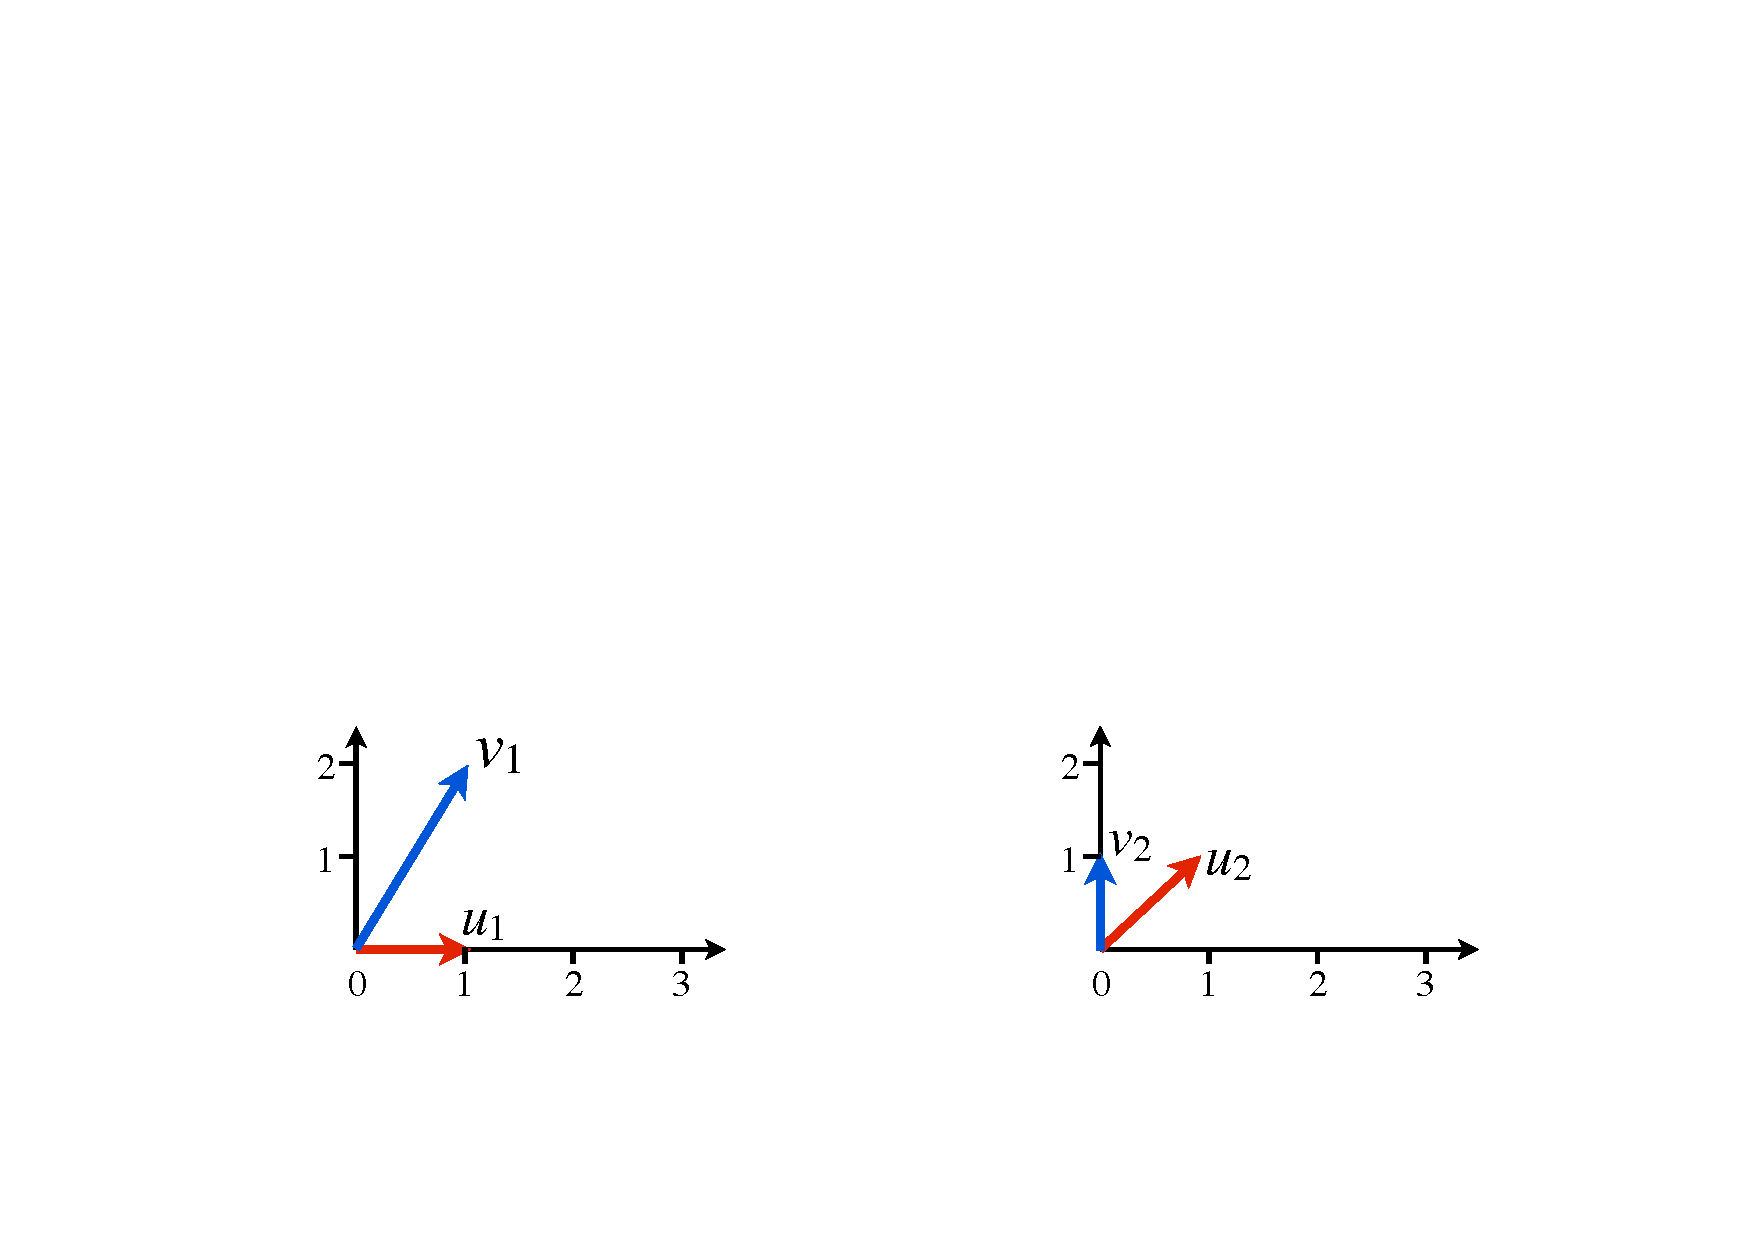
\includegraphics[width=0.6\textwidth]{fig.pdf}
\end{question}


\subsection*{Insight}

% Question 35
\begin{question}
A clique is  a fully connected subset of nodes in a graph. 
A maximal clique is a clique which is not a subset of a larger clique.
Consider now the graph below, where the $X_i$ are the nodes.  What are the maximal cliques? 
\begin{center}
\scalebox{0.75}{
\hskip1.4cm
\begin{tikzpicture}[ugraph]
%\node[font=\Large] at (1.2,2.8) {Undirected Graph};
\node[cont] (x1) at (0,2) {$X_1$};
\node[cont] (x2) at (2,2) {$X_2$};
\node[cont] (x3) at (2,0) {$X_3$};
\node[cont] (x4) at (0,0) {$X_4$};
\node[cont] (x5) at (3,1) {$X_5$};
\draw(x1) -- (x2);\draw(x1) -- (x3); \draw(x1) -- (x4);
\draw(x2) -- (x3); \draw(x2) -- (x4);
\draw(x3) -- (x4); \draw(x2)--(x5);\draw(x3)--(x5);
\end{tikzpicture}}
\end{center}

% TODO (Behrouz) Find out how to present the solution. The natural way to do so would be to have a two-part question with the second depending on the solution of first. Is that possible to do in ximera?

% TODO (Behrouz) The solution is an unordered set. Could that be specified in ximera?

\begin{solution}
The cliques are \answer {($X_1$,$X_2$,$X_3$,$X_4$) and ($X_2$,$X_3$,$X_5$)}.
\end{solution}
\end{question}

% Question 36
\begin{question}
Consider the following definitions.  
A vertical bar separates alternatives. For instance, $gray  \mid grey$ defines the set \{$gray$, $grey$\}.
Parentheses are used to define the scope and precedence of the operators (among other uses). For example, $gray \mid grey$ and $gr(a\mid e)y$ are equivalent patterns which both describe the set 
 \{$gray$, $grey$\}.
The quantifier $^*$ denotes that the previous element may be repeated zero or more times. 
 For example, $ab^*c$ includes $ac$, $abc$, $abbc$, $abbbc$, and so on.

Does the set $d (a \mid bc)^*t  $ include $dat$, $daaaaat$, $dbcabct$ ?  

\begin{solution}
\begin{multiple-choice}
\choice[correct] {yes}
\choice {no}
\end{multiple-choice}
\end{solution}
 
All three strings match the given expression:
\begin{align*}
&d \, \underline{a} \, t\\
&d \, \underline{a} \, \underline{a} \, \underline{a} \, \underline{a} \, \underline{a} \, t\\
&d \, \underline{bc} \, \underline{a} \, \underline{bc} \, t
\end{align*}

How would you define the set of all binary representations of natural numbers (i.e., 0, 1, 10, 11, ... ) ?

\begin{solution}
The answer is \answer{$0 | (1(0|1)*)$}.
\end{solution}
\end{question}

\end{document}